% cpedoc.tex V2.0, 13 May 2010

\documentclass[times]{cpeauth}

\usepackage{moreverb}
\usepackage{xspace}

\newif\ifdraft
\drafttrue
\ifdraft
\newcommand{\onote}[1]{ {\textcolor{cyan} { (***Ole: #1) }}}
\newcommand{\terminology}[1]{ {\textcolor{red} {(Terminology used: \textbf{#1}) }}}
\newcommand{\owave}[1]{ {\cyanuwave{#1}}}
\newcommand{\jwave}[1]{ {\reduwave{#1}}}
\newcommand{\alwave}[1]{ {\blueuwave{#1}}}
\newcommand{\jhanote}[1]{ {\textcolor{red} { ***shantenu: #1 }}}
\newcommand{\alnote}[1]{ {\textcolor{green} { ***andreL: #1 }}}
\newcommand{\amnote}[1]{ {\textcolor{blue} { ***andreM: #1 }}}
\newcommand{\smnote}[1]{ {\textcolor{brown} { ***sharath: #1 }}}
\newcommand{\pmnote}[1]{ {\textcolor{brown} { ***Pradeep: #1 }}}
\newcommand{\msnote}[1]{ {\textcolor{cyan} { ***mark: #1 }}}
\newcommand{\note}[1]{ {\textcolor{magenta} { ***Note: #1 }}}
\else
\newcommand{\onote}[1]{}
\newcommand{\terminology}[1]{}
\newcommand{\owave}[1]{#1}
\newcommand{\jwave}[1]{#1}
\newcommand{\alnote}[1]{}
\newcommand{\amnote}[1]{}
\newcommand{\athotanote}[1]{}
\newcommand{\smnote}[1]{}
\newcommand{\pmnote}[1]{}
\newcommand{\jhanote}[1]{}
\newcommand{\msnote}[1]{}
\newcommand{\note}[1]{}
\fi

\newcommand{\pilot}{Pilot\xspace}
\newcommand{\pilots}{Pilots\xspace}
\newcommand{\pilotjob}{Pilot-Job\xspace}
\newcommand{\pilotjobs}{Pilot-Jobs\xspace}
\newcommand{\pilotcompute}{Pilot-Compute\xspace}
\newcommand{\pilotmapreduce}{PilotMapReduce\xspace}
\newcommand{\pilotdata}{Pilot-Data\xspace}
\newcommand{\pd}{PD\xspace}
\newcommand{\pj}{PJ\xspace}
\newcommand{\pjs}{PJs\xspace}
\newcommand{\pds}{Pilot Data Service\xspace}
\newcommand{\computeunit}{Compute-Unit\xspace}
\newcommand{\computeunits}{Compute-Units\xspace}
\newcommand{\dataunit}{Data-Unit\xspace}
\newcommand{\dataunits}{Data-Units\xspace}
\newcommand{\du}{DU\xspace}
\newcommand{\dus}{DUs\xspace}
\newcommand{\cu}{CU\xspace}
\newcommand{\cus}{CUs\xspace}
\newcommand{\su}{SU\xspace}
\newcommand{\sus}{SUs\xspace}
\newcommand{\schedulableunit}{Schedulable Unit\xspace}
\newcommand{\schedulableunits}{Schedulable Units\xspace}
\newcommand{\cc}{c\&c\xspace}
\newcommand{\CC}{C\&C\xspace}

\usepackage[
%dvips,
colorlinks,bookmarksopen,bookmarksnumbered,citecolor=red,urlcolor=red]{hyperref}

\newcommand\BibTeX{{\rmfamily B\kern-.05em \textsc{i\kern-.025em b}\kern-.08em
T\kern-.1667em\lower.7ex\hbox{E}\kern-.125emX}}

\def\volumeyear{2012}



\begin{document}

\runningheads{S. Jha et al.}{Pilot-Abstractions for MapReduce-based  Cloud Applications}

\title{Pilot-Abstractions for MapReduce-based Cloud Applications}

%on Clouds and Grids}

%Extensible, Scalable, Interoperable 

\author{Andre Luckow, Pradeep Mantha, Melissa Romanus, Shantenu
  Jha\corrauth}

\address{Radical Research Group, Rutgers University}

\corraddr{Journals Production Department, John Wiley \& Sons, Ltd,
The Atrium, Southern Gate, Chichester, West Sussex, PO19~8SQ, UK.}

\begin{abstract}

The data generated by scientific applications is experiencing an
exponential growth; there exists a risk that the ability to analyze it
successfully may lag. Efficient and integrated analytical capabilities
that support scalable and advanced analytics whilst supporting
interoperability and extensibility are required; this includes runtime
environments and methods that can exploit them.  In addition to being
effective on localized data, MapReduce can when used in conjunction
with appropriate runtime environments, be used to efficiently process
distributed data across a distributed set of resources.  Specifically,
in recent work we demonstrated precisely such capabilities, viz.,
showed how Pilot-MapReduce --- a flexible, infrastructure-independent
runtime environment for MapReduce was able to address the
data-analytic requirements for a large-scale problem for both local
and distributed data.  PMR is based on Pilot-abstractions for compute
(Pilot-Jobs) and data (Pilot-Data). Pilot-Jobs are used to couple the
map phase computation to the nearby source data, and Pilot-Data is
used to move intermediate data using parallel data transfers to the
reduce computation phase.  This work builds upon earlier work to show
how Pilot abstractions and PMR enable the processing of distributed
data across multiple heterogeneous distributed infrastructure,
including concurrent usage of clouds and traditional
grids/clusters. We further show how PMR can efficiently support
different infrastructure and application characteristics, We further
analyze different resource topologies and MapReduce configuration,
such as both hierarchical and iterative MapReduce. In particular, we
investigate typical infrastructure trade-offs (e.g. the overhead times
in spawning virtual machines, the geographic distribution, etc).

\end{abstract}

\keywords{MapReduce; Grid Computing; Cloud Computing; K-Means; Data-Intensive; Compute-Intensive}

\maketitle

\footnotetext[2]{Please ensure that you use the most up to date
class file,
available from the CPE Home Page at\\
\href{http://www3.interscience.wiley.com/journal/117946197/grouphome/home.html}{\texttt{http://www3.interscience.wiley.com/journal/117946197/grouphome/home.html}}}

\vspace{-6pt}

\section{Introduction}
\vspace{-2pt}

\jhanote{In general: no references in abstract: \pilotmapreduce
  (PMR)~\cite{Mantha:2012:PEF:2287016.2287020} } \jhanote{last few
  sentences of abstract need fixing}


\begin{verbatim}

Application perspective versus Infrastructure perspective: (I)
 Application Motivation/Challenges: Scaling data intensive
 applications - Why is this a problem? Any real application requires
 this problem to be solved?  - CMS, Atlas generates PBs of data/ day.
  (II) Infrastructure Motivation: Emerging infrastructure, data
 oriented infrastructure, scalability of infrastructure, possibly
 better abstractions and capabilities.

Note our focus and context: (i) distributed data scenarios (ii) pilot
 abstraction to address heterogeneity, scalability and extensibilty

Some Research Questions: (i) How does Pilot-Abstraction work in the
 clouds (we've addressed pilot-jobs before, now focus on pilot-data)
 (ii) how to address data distribution in the cloud? (iii) cloud data
 localization requirements: how and when does that become a barrier?
  (iv) related to previous, Can we say something when to use cloud or
 When Grid?

\end{verbatim}

\jhanote{Other Issues worth mentioning: not sure what these are tying
 to say: Does minimizing queue wait time, distributed nature of
 Pilot-abstractions motivate Domain Scientists to use freely available
 Grid resources?  Waiting time and cost increases as Number of
 instances required increase?  HOw is it beneficial than Grids?}


\note{Why Domain scientists are moving to cloud? Hype? Due to
  non-availability of necessary simple abstractions to scale
  applications on Grid?} \jhanote{I don't think we should be making
    that argument here for it undermines our own point of view that
    Pilot abstractions have been relatively / modestly successful on
    grids}

\note{These are design objectives: Interoperability, Scalability,
  Extensibility/Flexibility/usability}

\note{Not in scope any more: Why Iterative MapReduce?What
  Application?  ( k-means?)Why k-means?  - twister mapreduce used
  k-means?  - k-means implemented using windows azure}


\section{Related Work}

Prior Work (Pradeep)

Related Work (Melissa)



\section{Cloud Computing and Cloud-based Infrastructures}

At a high level, cloud computing is defined by Mell/Grance~\cite{nist_cloud}
as a model for enabling convenient, on-demand network access to a shared pool
of configurable computing resources (e.g., networks, servers, storage,
applications, and services) that can be rapidly provisioned and released with
minimal management effort or service provider interaction.

\alnote{Do we want to talk about the ``old'' SaaS, PaaS and IaaS stuff?}

\subsection{Commercial Clouds}

\subsection{Science Clouds}

\subsection{Cloud APIs}

Amazon API
GData API
OpenStack API
OCCI



\subsection{Data-intensive Application and Clouds}

In distributed settings, storage is often a black box for the application with
unknown quality of services, i.\,e. the application usually does not know what
bandwidths and latencies it can expect. Furthermore, physical and logical
distribution implies higher penalties for inefficient data access as the data
traverses several hardware and software layers.

In general, different types of storage exist (see figure~\ref{fig:figures_storage-types}):

\begin{enumerate}
	\item \textbf{Local Storage:} describes local hard disk directly attached 
	to the compute resource.
	\item \textbf{Network Filesystem:} refers to different forms of 
	distributed (possible parallel) filesystems. The filesystem is commonly 
	exported via the Posix API and a virtual filesystem layer.
	\item \textbf{Distributed Storage:} refers to a highly distributed type of 
	storage systems that spawn across multiple data centers. Access to such 
	storage systems via a common -- often simplified -- namespace and API. For 
	example, cloud systems, such as the Azure Blob Storage, Amazon S3 and 
	Google Storage, provide only a namespace with a 1-level hierarchy. 
\end{enumerate}

While the coupling between compute and data in type 1 and 2 is very high, it 
is only small in the later case. In general, the buffer type 3 storage are 
more optimized to reliably storing large volumes of data and achieving high
read throughputs.

\subsubsection{Hadoop in the Cloud}

\alnote{How do the different cloud providers chose to re-package Hadoop and 
provide an integrated service?}

\begin{itemize}
	\item Elastic MapReduce
	\item Hadoop on Azure
\end{itemize}

\alnote{Why do we exclude databases?}

\begin{figure}[t]
	\centering
		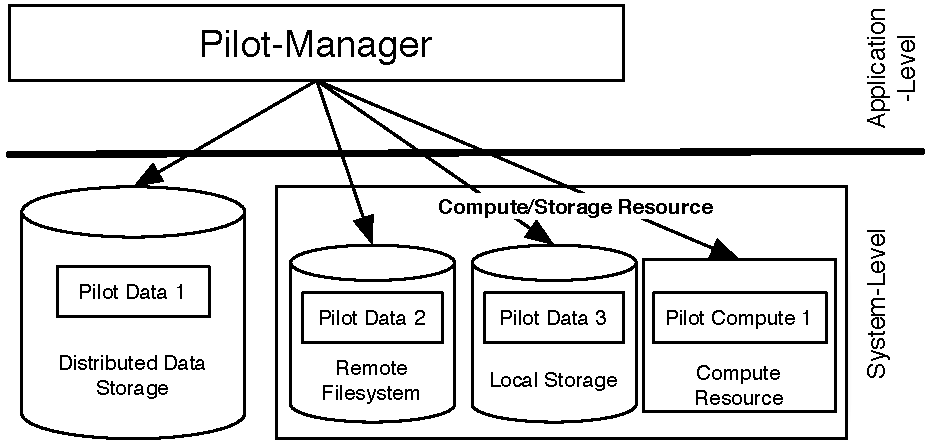
\includegraphics[width=0.7\textwidth]{figures/storage-types.pdf}
	\caption{Pilot-Compute and Pilot-Data on Different Types of Storage Resources}
	\label{fig:figures_storage-types}
\end{figure}

Table~\ref{tab:storage-systems} shows an overview of distributed storage 
systems. The focus of this analysis are file-based storage systems. Structured
storage types (e.g. relational databases) and key-/values stores are not 
considered.

\begin{table}[t]
\centering
\begin{tabular}{|p{1.7cm}|p{1.3cm}|p{1.3cm}|p{1.3cm}|p{1.4cm}|p{1.4cm}|p{1.3cm}|p{1.2cm}|}
	\hline
	\textbf{Storage Type} &\textbf{Azure} &\textbf{Amazon} &\textbf{Google} &\textbf{Open\-Stack} &\textbf{Euca\-lyptus} &\textbf{XSEDE}  &\textbf{OSG} \\
	\hline
	Local	&yes &yes &yes &yes &yes &yes &yes\\
	\hline
	Network Filesystem &Azure Drive &EBS &GCE Block Storage &Nova Volumes &? &Lustre, GPFS 
	&no\\
	\hline
	Distributed Storage &Azure Blob Storage &S3 &Google Storage &Swift & Walrus &GFFS
	 &SRM\\
	\hline	
\end{tabular}
\caption{File-based storage types for different infrastructures (key/value and 
SQL-based storage types omitted) \label{tab:storage-systems}}
\end{table}


\section{Pilot Abstractions and Clouds}

% Intro to P* model

\begin{figure}[t]
	\centering
		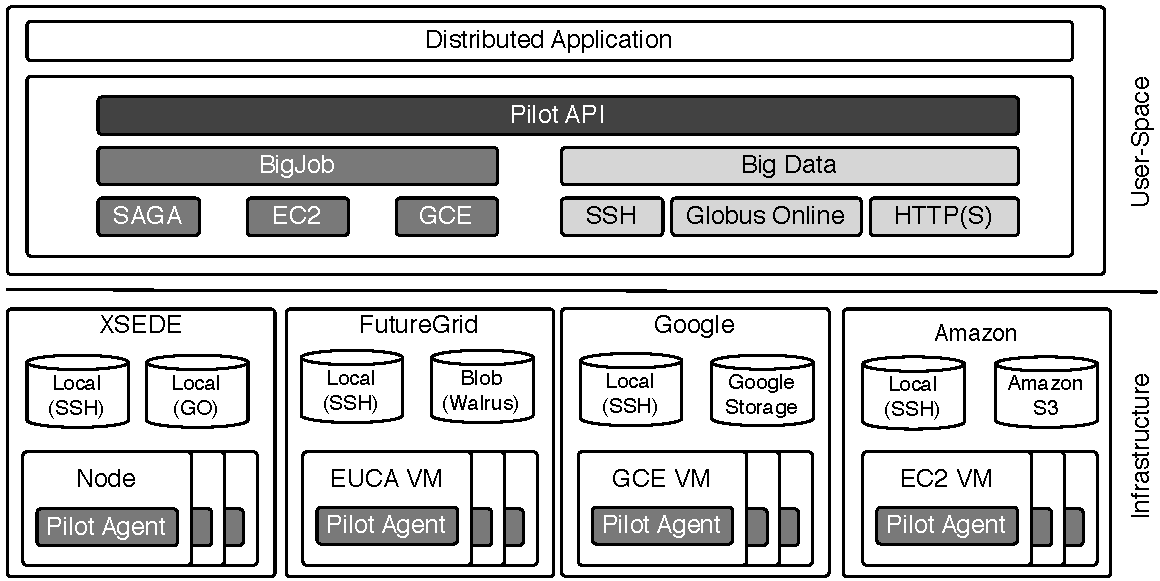
\includegraphics[width=0.7\textwidth]{figures/cloud_pilot_job.pdf}
	\caption{Pilot Abstractions and Clouds\alnote{todo: differentiate between 
	storage and transfer protocol}}
	\label{fig:figures_cloud_pilot_job}
\end{figure}

Figure~\ref{fig:figures_cloud_pilot_job} shows how the Pilot-API and 
BigJob/BigData can be used to manage a heterogenous set of both cloud and grid 
resources. BigJob supports various resource types via a flexible plugin 
architecture. In addition to SAGA, BJ can natively utilize both the EC2 and 
GCE API to launch BJ agents. Similarly, BigData supports various data access
protocols and storage types -- currently, SSH, Globus Online, Google Storage
and Amazon S3.

Figure~\ref{fig:figures_data-flow} shows the interactions and the data flow 
between Pilot Computes and Data.
\begin{figure}[htbp]
	\centering
		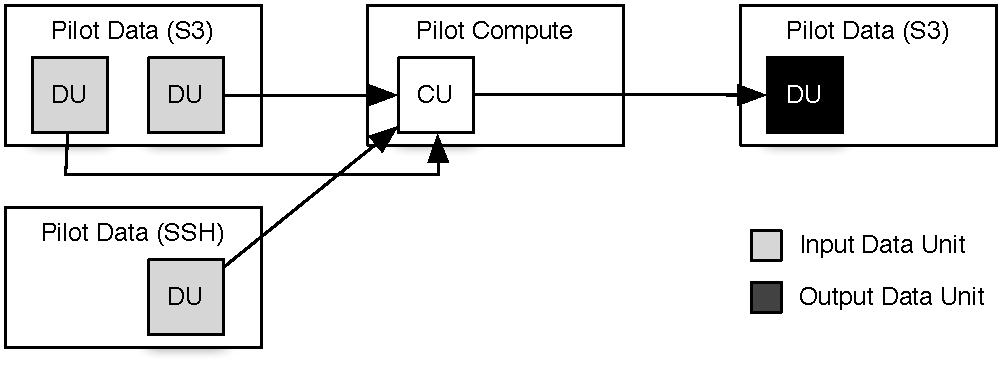
\includegraphics[width=0.7\textwidth]{figures/data-flow.pdf}
	\caption{DU and CU Interactions and Data Flow}
	\label{fig:figures_data-flow}
\end{figure}



\section{Pilot-MapReduce}
Pilot-MapReduce is a pilot-based implementation of the MapReduce
programming model, which decouples the logic/pattern of MapReduce from
the actual management of the compute, data and network resources. By
decoupling job scheduling and monitoring from the resource management,
PMR can efficiently reuse the resource management and late-binding
capabilities of BigJob and BigData.

PMR exposes an easy-to-use interface which provides the complete
functionality needed by any MapReduce-based application, while hiding
the more complex functionality, such as chunking of the input, sorting
the intermediate results, managing and coordinating the map and reduce
tasks, etc., these are generically implemented by the
framework~\cite{pmr2012}.

\section{Experiments}

\subsection{Infrastructure}

Compute:
\begin{itemize}
	\item FutureGrid/XSEDE: Sierra, Kraken 
	\item FutureGrid India/Eucalyptus
	\item FutureGrid India/OpenStack
\end{itemize}

Data:

	
\subsection{Word Count}

Experiments:
\begin{itemize}
	\item  Scale input data: 1GB, 10GB, 100GB, 1000 GB
	\item  Different amounts of intermediate data: 1GB, 10GB, 100GB, 1000 GB
	\item  Number of Resources: 1, 2, 4, 8, 16, 32 VMs
\end{itemize}

\subsection{NGS}

\section{Conclusion and Future Work}

\bibliographystyle{wileyj}
\bibliography{literatur,saga,saga-related,local}

\end{document}
